\chapter{Background}
\label{chapter:background}

This section briefly introduces relevant concepts of machine learning and deep learning to better familiarize the reader with the methodology and techniques as well as contextualize the state-of-the-art work that will be reviewed later in chapter \ref{chapter:sota}.

\section{Supervised Learning}

A supervised learning problem is a machine learning problem in which the data has the correct expected output for every input.

More formally, it is a problem in which there are $m$ labeled pairs $(x^{(i)}, y^{(i)})$, also denoted as samples, where $x^{(i)} \in \mathbb{R}^n$ (i.e. the input vectors, commonly referred to as features) and $y^{(i)} \in \mathbb{R}^n$ (i.e. the corresponding output vector, usually called the target or label) which have some relationship expressed by some function.

The goal of supervised learning is to find a function $h_{\theta}(x)$ (sometimes called the hypothesis) that usefully approximates the true function in the underlying relationship between the input $x$ and associated output $y$, parameterized by $\theta$.

In supervised learning, the data samples are commonly split into three separate sets with different intents and used exclusively for that purpose:

\begin{itemize}
    \item Training Set: samples used for actually fitting the model's parameters (e.g. weights and biases of a neural network);
    \item Validation Set: samples used to select the best model by testing different sets of hyperparameters or architectures;
    \item Test Set: samples used to assess the final performance of the final model.
\end{itemize}

It is important to follow this taxonomy carefully and not use the different sets for the different tasks interchangeably. As \citeauthor{crossvalidationbias} point out in their \citeyear{crossvalidationbias} paper, if, for example, we use the test set to simultaneously tune hyperparameters and assess its generalization performance we risk optimistically biasing the model. As such, if we use any one set to tune hyperparameters, we must use a different set for evaluation to get an unbiased assessment of the model's generalization performance.

However, this technique (typically referred to as the holdout method) has its downsides:

\begin{itemize}
    \item using an arbitrary fixed split of the dataset means that we are completely setting aside data for validation and testing which will not be used for fitting the model and vice versa, thus wasting data in some sense
    \item without averaging over multiple runs (i.e. different splits) with different initial conditions, results may be biased and misleading
\end{itemize}

$K$-fold cross-validation is a common cross-validation technique that randomly partitions the data into $K$ equally sized subsamples, of which a single subsample is used for testing and the remaining $K-1$ subsamples for fitting the model, a process which is repeated $K$ times to yield $K$ performance estimations that can be averaged over to produce one estimation that can be referred to. In this way all samples are used for training and testing, which is an advantage over repeated random sub-sampling which does not systematically use all samples for training and testing.

Nested cross-validation techniques are required when, in addition to estimating a model's generalization performance (i.e. performance on the test set), it is also necessary to select the best model among many (e.g. with different hyperparameters) \cite{crossvalidationbias}. A truly nested variant will use an inner loop of $L$ folds to tune the hyperparameters and select the best model, and an outer loop of $K$ folds to evaluate the models selected by the inner loop. A simpler (albeit not really nested) scheme is one that is similar to the $K$-fold cross-validation we described above, except that, of the $K$ equally sized subsamples, we take 1 subsample for validation, another 1 subsample for testing, and the remaining $K-2$ subsamples are used for training. However, in practice, nested cross-validation when selecting classifiers is overzealous and too expensive for most applications \cite{nestedcvoverzealous}.


\section{Binary Classification}

In general, let

\begin{itemize}
    \item $L \colon \mathbb{R}^n \to \mathbb{R}$ be a function, called the loss function, which quantifies the quality of a particular set of parameters $\theta$ relative to a single data sample $(x^{(i)}, y^{(i)})$;
    \item $J \colon \mathbb{R}^n \to \mathbb{R}$ be a function, called the cost function, which quantifies the quality of a particular set of parameters $\theta$ relative to all the $m$ samples in the training set. $$J(\theta) = \frac{1}{m} \sum_{i=1}^{m} L(h_{\theta}(x^{(i)}), y^{(i)})$$
\end{itemize}

In particular, the linear regression cost function can be easily understood as the summation of the differences between the predictions and the ground truth labels:

$$
J(\theta) = \frac{1}{2m} \sum_{i=1}^{m} (h_{\theta}(x^{(i)}) - y^{(i)})^2
$$

In a binary classification problem specifically we have that $y^{(i)} \in \{0, 1\}$. Unfortunately, as it turns out, the linear regression cost function is unsuitable for binary classification because it would be a non-convex function with many local minima, which in turn would make optimization very difficult.

Essentially, binary classification requires a cost function that penalizes very confident wrong predictions while also rewarding confident right predictions, i.e.,

\begin{itemize}
    \item if the prediction is $h_{\theta}(x) = 0$ and the ground-truth label is $y = 0$, $J(\theta)$ is low;
    \item if the prediction is $h_{\theta}(x) = 0$ and the ground-truth label is $y = 1$, $J(\theta)$ is high;
    \item if the prediction is $h_{\theta}(x) = 1$ and the ground-truth label is $y = 0$, $J(\theta)$ is high;
    \item if the prediction is $h_{\theta}(x) = 1$ and the ground-truth label is $y = 1$, $J(\theta)$ is low.
\end{itemize}

Whereas in linear regression the hypothesis is of the form $h_{\theta}(x) = \theta^Tx$, in binary classification (or logistic regression) the hypothesis is of the form $h_{\theta}(x) = \sigma(\theta^Tx)$ to squash predictions to the interval $[0, 1]$, hence the name logistic regression, because it uses the sigmoid-shaped logistic function $\sigma(z) = \frac{1}{1 + e^{-z}}$.

A useful loss function (sometimes called binary cross-entropy in some literature) for logistic regression that takes these requirements into consideration is

$$
L(h_{\theta}(x^{(i)}), y^{(i)}) =
\begin{dcases}
    -\log(h_{\theta}(x^{(i)})),& \text{if } y^{(i)} = 1\\
    -\log(1 - h_{\theta}(x^{(i)})),& \text{if } y^{(i)} = 0
\end{dcases}
$$

or, cleverly arranging things algebraically,

$$
J(\theta) = -\frac{1}{m} \sum_{i=0}^{m} ( y^{(i)}\log(h_{\theta}(x^{(i)})) + (1 - y^{(i)})\log(1 - h_{\theta}(x^{(i)})) )
$$

\subsection{Evaluation}

To evaluate a binary classifier means to compare the model's predicted conditions against the true conditions, where one must consider:

\begin{itemize}
    \item \ac{TP}, cases correctly classified as positive, i.e. $h(x^{(i)}) = 1$ matches $y^{(i)} = 1$;
    \item \ac{TN}, cases correctly classified as negative, i.e. $h(x^{(i)}) = 0$ matches $y^{(i)} = 0$;
    \item \ac{FP}, cases incorrectly classified as positive, i.e. $h(x^{(i)}) = 1$ but $y^{(i)} = 0$;
    \item \ac{FN}, cases incorrectly classified as negative, i.e. $h(x^{(i)}) = 0$ but $y^{(i)} = 1$.
\end{itemize}

From these basic measurements one can derive useful metrics:

\begin{itemize}
    \item \ac{TPR}, also known as sensitivity or recall, is basically the percentage of actual positives that are correctly identified as positive;
        $$TPR = \frac{TP}{TP + FN}$$
    \item \ac{TNR}, also known as specificity, is the percentage of actual negatives that are correctly identified as negative;
        $$TNR = \frac{TN}{FP + TN}$$
    \item \ac{PPV}, also known as precision,
        $$PPV = \frac{TP}{TP + FP}$$
    \item \ac{NPV}
        $$NPV = \frac{TN}{TN + FN}$$
    \item \ac{FPR} is the percentage of actual positives that are incorrectly identified as negative;
        $$FPR = 1 - TNR$$
\end{itemize}

As a summary statistic one can derive the accuracy $A$ as the percentage of total items classified correctly

$$
A = \frac{TP + TN}{TP + FP + TN + FN}
$$

However accuracy is misleading in cases where there is a class imbalance because a model can always predict the value of the majority class and still report a high accuracy value despite missing all predictions in the minority class. Instead F1 score should be preferred. F1 score is the harmonic mean of precision and recall given by

$$
F_1 = 2 \times \frac{PPV \times TPR}{PPV + TPR}
$$

Lastly, \ac{AUC} is known as the area under the \ac{ROC} curve, i.e. the area under the plot of \ac{FPR} versus \ac{TPR} at different points in the interval $[0, 1]$.

\subsection{Class Imbalance}

In binary classification problems, it is said that a dataset of $m$ samples has class imbalance when there is a majority class with $|S_{maj}|$ samples and a minority class with $|S_{min}|$ samples where $|S_{maj}| > |S_{min}|$, in other words when there is a significant difference between the number of samples of one class compared to the other. It is very common to see datasets in which classes are highly imbalanced, simply because it reflects the real world distribution (e.g. there are more benign moles than actual melanoma cases). A lot of machine learning algorithms do not perform well under this imbalance. When a dataset is imbalanced, machine learning algorithms will typically over-classify the majority group due to its increased prior probability. Thus, the samples in the minority group are misclassified more often than the majority group \cite{Johnson2019}.

\citeauthor{haibo2009} provide a comprehensive survey of class balancing algorithms \cite{haibo2009}, of which oversampling of the minority class is the simplest and most natural. In practice the minority class must be oversampled by a factor (i.e. number of transformations applied to each original sample) of $\frac{|S_{maj}|}{|S_{min}|}$. Sometimes, perhaps because of an overfitting problem, it is also necessary to augment the total number of samples $m$ to a new total number of samples $m'$, in which case

\begin{itemize}
    \item the minority class must be oversampled by augmenting its samples  by a factor of $\frac{\frac{m'}{2}}{|S_{min}|}$
    \item and the majority class must also be augmented by a factor of $\frac{\frac{m'}{2}}{|S_{maj}|}$
\end{itemize}

\section{Optimization}

Given a cost function $J$ and initial parameters $\theta$, the goal is to find the optimal $\theta^*$ that minimizes the cost function, i.e. the optimization objective is

$$
\theta^{*} = \argmin_{\theta} J(\theta)
$$

In the deep learning high-dimensional optimization landscape, the objective function is highly non-convex w.r.t. the parameters, so one can't use any of the tools from the convex optimization literature. Using calculus to find the minimum analytically is only feasible for trivial, low-dimensional, convex functions.

\subsection{Brute-force Search}

A naive first approach is to systematically and exhaustively enumerate and evaluate many candidate solutions while keeping track of the best one. This simple solution, arguably the simplest metaheuristic, is infeasible in the context of deep neural networks due to the curse of dimensionality.

\subsection{Random Optimization}

Rather than try all solutions exhaustively, another approach is to try random values of $\theta$ in a loop and record the running best until some stopping criteria.

\subsection{Random Local Search}

A slightly better strategy is to start with random $\theta$ and iteratively refine the best-found solution (hence the local in local search) until some stopping criteria.

\subsection{Gradient Descent}

Random local search forms a good basis for optimization, but there is no need to move randomly in search-space. The negative of the gradient of the cost function w.r.t. the parameters $\theta$ over all $m$ training samples gives the direction of steepest descent (i.e. the direction in which the cost function decreases):

$$
\nabla_{\theta} J(\theta) = \frac{1}{m} \sum_{i=1}^{m} \nabla_{\theta} L(h_{\theta}(x^{(i)}), y^{(i)})
$$

A parameter $\eta \in \mathbb{{R}^{+}}$, called the learning rate, controls the size of the step to take in the direction of the gradient. The learning rate $\eta$ must be set carefully to ensure that the cost function converges. A small enough value will ensure convergence, but requires a larger number of updates to get there, whereas bigger values will likely result in divergence.

Thus emerges a very simple and natural update rule (called batch gradient descent) for our parameters:

$$
\theta^{t+1} = \theta^t - \eta \nabla_{\theta} J(\theta)
$$

Computing the gradient $\nabla J$ with respect to the original $m$ training samples is computationally and memory intensive for very big $m$. But it turns out we can get a good estimate of the true gradient $\nabla J$ by averaging over a smaller random number of samples $m'$, i.e.,

$$
\frac{\sum_{i=1}^{m'} \nabla J_i}{m'} \approx \frac{\sum_{i=1}^m \nabla J_{i}}{m} \approx \nabla J
$$

This idea is interchangeably referred to as mini-batch gradient descent or \ac{SGD} (in some literature only when $m' = 1$).

More recently, gradient descent methods have been further developed to find individual learning rates per parameter which are adapted using estimations of the first and second moments of the gradient. \citeauthor{ruder2016} \cite{ruder2016} presents an extensive review of these adaptive variations of gradient descent. Despite the popularity of these methods, sometimes they offer marginal value versus the classic \ac{SGD}. Wilson et al. \cite{wilson2017} show that the solutions found by adaptive methods usually generalize worse when compared to \ac{SGD}, which suggests that machine learning practicioners should reconsider the use of adaptive methods and try other methods too.

\section{Initialization}

An optimization algorithm like gradient descent is inherently iterative in its update rule (for iterations $t > 0$)

$$
\theta^{t+1} = \theta^t - \eta \nabla_{\theta} J(\theta)
$$

for which we need to initialize the matrix $\theta^0$ such that the first update works. This initialization determines how quickly optimization converges or whether it converges at all, which is why it is so important.

A reasonable first approach would be to initialize all values of the matrix $\theta$ to zero. However, e.g. in a neural network this does not have any symmetry breaking properties because if every weight is initialized to zero then every neuron will compute the same activation (assuming all neurons use the same activation function), thus the gradients computed by backpropagation will also be the same and result in the exact same updates during gradient descent. Therefore parameters must be chosen in such a way that they break this symmetry, which is what motivates the use of random initialization. However simply drawing random parameters (e.g. from a Gaussian distribution with mean 0 and standard deviation 1) might result in too small or too big parameter values and very wide in range which originate a vanishing or exploding gradient problem where different layers effectively learn at different speeds.

Modern initialization techniques are heuristic based and designed around the activation functions themselves to counter these problems by, essentially, guaranteeing the activations' mean to be $0$ and the variance to be the same across different layers. Under these conditions the backpropagated gradient will not be multiplied by very small or very big values (which would lead to vanishing or exploding gradient problems, respectively). Specifically,

\begin{itemize}
    \item for tanh activation functions, Xavier et al. \cite{xavierinit} recommend drawing parameters from either $\mathcal{N}(0, \frac{1}{n_{in}})$ or $\mathcal{N}(0, \frac{2}{n_{in}+n_{out}})$ where $n_{in}$ is the number of input neurons and $n_{out}$ the number of output neurons in that layer;
    \item for ReLU activation functions, He et al. \cite{heinit} suggest drawing from $\mathcal{N}(0, \frac{2}{n_{in}})$.
\end{itemize}

More recently, initializing a network with parameters transferred from other networks (typically trained on natural image datasets whose lower-layers' features generalise well to other tasks) has emerged as a very useful and pragmatic initialization strategy which in practice works very well for most tasks \cite{howtransferable}, giving birth to what is now known as transfer learning.

\section{Feature Scaling}

Some machine learning algorithms rely on the distance between the features in a feature vector $x$ and assume the values are on the same scale. Min-max normalization rescales $x$ to $x'$ to be on the interval $[0, 1]$, i.e.

$$
x' = \frac{x - \min{(x)}}{\max{(x)} - \min{(x)}}
$$

Other machine learning algorithms assume that the feature vector $x$ follows a Gaussian distribution (i.e. zero mean and unit-variance). Standardization (sometimes more intuitively called normalization) is the process of rescaling $x$ (where $\mu_x$ is the mean of each feature vector $x$ and $\sigma_x$ its standard deviation) to $x'$ to follow a Gaussian distribution, i.e.

$$
x' = \frac{x - \mu_x}{\sigma_x}
$$

In practice, gradient descent converges much faster with features that follow a normal distribution \cite{batchnormalization}.


\section{Bias-Variance Tradeoff}

The goal of supervised learning is to find a function $\hat{f}(x)$ that approximates the true function $f(x)$ in the underlying relationship between the data $x$ and associated labels $y$. For this approximation to be useful it should simultaneously

\begin{itemize}
    \item accurately capture the training data
    \item generalize to new data
\end{itemize}

It turns out this is very difficult to do simultaneously. Decomposition of the expectation $E$ of the error on an unseen sample $x$ yields

$$
{\displaystyle {\begin{aligned}\operatorname {E} &={\Big (}\operatorname {Bias} {\big [}{\hat {f}}(x){\big ]}{\Big )}^{2}+\operatorname {Var} {\big [}{\hat {f}}(x){\big ]}+\sigma ^{2}\\\end{aligned}}}
$$

where

\begin{itemize}
    \item the bias of the approximation is the error caused by the simplifying assumptions inherent to the approximation
    \item the variance of the approximation is the error caused by how much the approximation $\hat{f}(x)$ will try to fit the data $x$ exactly
    \item the error $\sigma^2$ is the variance of the noise within the data, which forms a lower bound on the expected error since all other equated terms are necessarily non-negative and the error $\sigma^2$ is irreducible
\end{itemize}

This formulation causes a tradeoff that models must make between bias and variance among the following possible scenarios:

\begin{itemize}
    \item high-variance low-bias models represent the training data well but risk overfitting to noise
    \item low-variance high-bias models are simpler but risk underfitting the training data, failing to capture the underlying signal
\end{itemize}

An underfitting (low variance) problem can be identified when the training error is high and the validation error is roughly equally high, which can be fixed by

\begin{itemize}
    \item training with more features
    \item decreasing regularization
\end{itemize}

On the other hand, an overfitting (high variance) problem can be identified when the training error is high and the validation error is comparatively much higher, which can be fixed by

\begin{itemize}
    \item training with more data
    \item training with less features
    \item increasing regularization
\end{itemize}

\section{Regularization}

In the optimization literature, regularization is seen as a modification $J_R(\theta)$ to the original objective function $J(\theta)$ that penalises large parameter values $\theta$ using some criteria $R(\theta)$ such that

$$
J_R(\theta) = J(\theta) + R(\theta)
$$

This regularization penalty can be seen as a form of Occam's razor that prefers simpler functions. In a sense, this redefines the optimization goal to simultaneously

\begin{itemize}
    \item fit the training data well (i.e. the $J(\theta)$ term) and
    \item keep the parameters small (i.e. the $R(\theta)$ term).
\end{itemize}

In the case of L1 regularization, also known as Lasso Regression,

$$
R(\theta) = \lambda \sum_{j=1}^{n} |x_j|
$$

which in essence

\begin{itemize}
    \item penalizes the absolute value of parameters, which tends to shrink parameters to be close to zero;
    \item effectively does feature selection because some of the parameters can be zero;
    \item consequently produces sparse matrices of parameters, which can be relevant;
    \item generally produces simpler and interpretable models.
\end{itemize}

Whereas in the case of L2 regularization, also known as Ridge Regression,

$$
R(\theta) = \lambda \sum_{j=1}^{n} x_j^2
$$

which basically

\begin{itemize}
    \item penalizes the sum of squared parameters, which tends to shrink parameters to be close to zero;
    \item does not do feature selection and does not produce sparse matrices;
    \item generally produces more complex models.
\end{itemize}

In practice, we control the regularization strength via the $\lambda$ parameter. Put simply, in a high variance scenario (overfitting) we should increase $\lambda$ and in a high bias situation (underfitting) we should decrease $\lambda$.

More recently, Dropout \cite{dropout} is another regularization technique designed specifically to prevent neural networks from overfitting by randomly dropping neuron (and their connections) from the network during training which prevents complex co-adaptations on training data.

\citeauthor{regularizationsurvey} present a much broader and more modern view of regularization in machine learning in their \citeyear{regularizationsurvey} paper \cite{regularizationsurvey}, where they define regularization more abstractly as any technique that allows the model to generalize better (i.e. perform better on the test set). They go over implicit regularization via data augmentation, network architecture, and the optimization algorithm itself as well as various explicit regularization techniques that penalize large weights (e.g. L1 and L2 regularization).

\section{Neural Network}

Neural networks allow defining complex, non-linear hypotheses $h_\theta(x)$ with parameters $\theta$ that we can fit to data and are traditionally composed of several neurons (as illustrated in figure \ref{fig:neuralnetwork}).

\begin{figure}[ht]
    \centering
    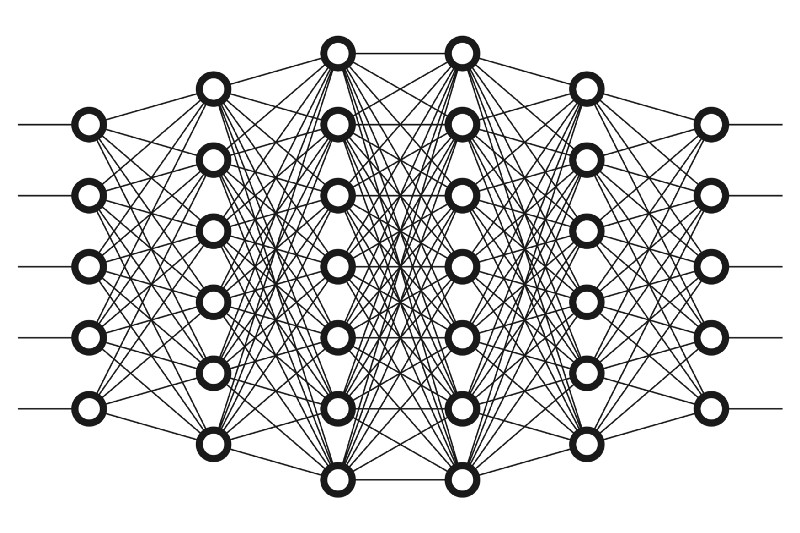
\includegraphics[width=0.6\textwidth]{figs/neuralnetwork.jpeg}
    \caption{Overly simplified view of a neural network composed of multiple neurons, in this case organized in an input layer, four fully-connected hidden layers, and an output layer. Source: datanami.com.}
    \label{fig:neuralnetwork}
\end{figure}

\subsection{Neuron}

A neuron is a computational unit parameterized by a weight matrix $W$ and bias vector $b$, which takes as input $x \in \mathbb{R}^{n}$ and outputs a hypothesis $h_{W,b}(x) = g(\sum^{i=1}_{n} W_{i}x_{i} + b) = g(W^Tx + b)$ that is activated by some (usually non-linear) function $g \colon \mathbb{R} \to \mathbb{R}$ called the activation function.

The activation function $g$ is what characterizes the neuron. If the activation function is the step function

$$
g(x) =
\begin{dcases}
    1,& \text{if } z \geq \theta\\
    0,& \text{if } z < \theta
\end{dcases}
$$

the neuron is reduced to the perceptron presented in 1950-1960 by \citeauthor{perceptron} \cite{perceptron}.

A sigmoid function is any bounded, differentiable, real function (e.g. logistic, tanh).

$$
g(x) = \frac{1}{1 + e^{-x}}
$$

ReLU is the abbreviation of rectified linear unit, which applies the non-saturating activation function $g(x)=\max(0,x)$. It effectively removes negative values from an activation map by setting them to zero. It increases the nonlinear properties of the decision function and of the overall network without affecting the receptive fields of the convolution layer. ReLU is preferred because it trains the neural network faster without a significant penalty to generalization accuracy.[62]

Other functions are also used to increase nonlinearity, for example the saturating hyperbolic tangent $g(x)=\tanh(x)$, $g(x)=|\tanh(x)|$, and the sigmoid function $\sigma (x)=(1+e^{-x})^{-1}$. \subsection{Forward Pass}
\label{subsection:forwardpass}

An $L$-layer neural network's activations can be recursively defined

$$
a^{l} =
\begin{dcases}
    f(W^{l-1}a^{l-1} + b^{l-1}),& \text{if } 1 < l \leq L\\
    x,              & \text{if } l = 1
\end{dcases}
$$

Let us also define the weighted inputs to the activation function, which is of importance when deriving the backpropagation equations.

$$
z^{l} = W^{l-1}a^{l-1} + b^{l-1}
$$

\subsection{Backward Pass}
\label{subsection:backwardpass}

Backpropagation is a way of computing the gradient through recursive application of the chain rule from calculus.

A network should be able to infer the right outputs given the right weights and biases. To learn these correct weights and biases, the network must be able to adjust them.

Small changes in weights $\Delta w_j$ and biases $\Delta b$ should only cause small changes in neuron output $\Delta a^L_i$. This is in fact the case. By the tangent line approximation

$$
\Delta a^L_i \approx \sum_j \frac{\partial a^L_i}{\partial w_j} \Delta w_j + \frac{\partial a^L_i}{\partial b} \Delta b
$$

Backpropagation is about understanding how changing the weights and biases in a network changes the cost function, which is precisely represented by $\frac{\partial C}{\partial w^l_{jk}}$ and $\frac{\partial C}{\partial b^l_j}$.

But to compute those, we first introduce an intermediate quantity, $\delta^l_j$, which we call the error in the $j$th neuron in the $l$th layer. Backpropagation will give us a procedure to compute the error $\delta^l_j$, which will then relate $\delta^l_j$ to $\frac{\partial C}{\partial w^l_{jk}}$ and $\frac{\partial C}{\partial b^l_j}$.


%% TODO: refactor, word engineering

The intuition behind the backpropagation algorithm is as follows. Given a training example $(x, y)$ we will first run a forward pass to compute all the activations throughout the network, namely the output of the network $h_{W,b}(x)$. Then, for each node $i$ in layer $l$, we would like to compute the error $\delta^{l}_i$ as a measure of how much that node was responsible for the error in the output $\delta^{L}_i$. For any of the nodes at the output of the neural network, this can be directly measured as the difference between the activation of a node and the labeled value.
The error that

Backpropagation relies on two important assumptions about the cost function:

\begin{itemize}
    \item it can be written as an average of cost per individual training sample $x$, i.e. $C = \frac{1}{m} \sum_x C_x$, because backpropagation can only compute $\frac{\partial C_x}{\partial w}$  and $\frac{\partial C_x}{\partial b}$ for a single training example $x$ which can then be averaged to obtain $\frac{\partial C}{\partial w}$  and $\frac{\partial C}{\partial b}$.
    \item it can be written as a function of the output at the neural network, i.e. $C = C(a^{L})$, which it otherwise
\end{itemize}

The error at the output layer $L$ is given by:

$$
\delta^L = \nabla_{a^L} C(a^L) \odot \sigma'(z^L)
$$

The error at an arbitrary hidden layer $l$ is given in terms of the error in layer $l+1$:

$$
\delta^l = ((w^{l+1})^T \delta^{l+1}) \odot \sigma'(z^L)
$$

Finally we can relate the error back to the gradient we wanted to compute:

$$
\frac{\partial C}{\partial b^l_j} = \delta^l_j
$$

$$
\frac{\partial C}{\partial w^l_{jk}} = a^{l-1}_k \delta^l_j
$$

The gradient descent update rules then become:

$$
1337
$$

\section{Convolutional Neural Network}

A \ac{CNN} is a class of deep, feed-forward artificial neural network, originally designed for computer vision problems where it is most popular. A \ac{CNN} consists of an input and an output layer, as well as multiple hidden layers. The hidden layers of a \ac{CNN} are typically comprised of:

\begin{itemize}
    \item Convolutional base composed by a stack of convolutional and pooling layers. Convolutional layers comprise a set of n independent filters which are independently convolved with the input volume to obtain an output volume of n feature maps. Pooling layers progressively reduce the spatial size of an input volume to reduce the amount of parameters and computation in the network. Pooling layers operate on each feature map independently. The main goal of the convolutional base is to generate features from the image.
    \item Classifier composed by fully connected layers. The main goal of the classifier is to classify the image based on the detected features. A fully connected layer is a layer whose neurons have full connections to all activation in the previous layer.
\end{itemize}

For a particular feature map (the output received on convolving the image with a particular filter is called a feature map), each neuron is connected only to a small chunk of the input image and all the neurons have the same connection weights.

Two key ideas in convolutional neural networks:

\begin{itemize}
    \item Parameter sharing is sharing of weights by all neurons in a particular feature map.
    \item Local connectivity is the concept of each neural connected only to a subset of the input image (unlike a neural network where all the neurons are fully connected)
\end{itemize}

This helps to reduce the number of parameters in the network and makes the computation more efficient.

To summarize, a convolutional layer:

\begin{enumerate}
    \item Accepts a volume of size $W_1 \times H_1 \times D_1$
    \item Requires four hyperparameters:
    \begin{enumerate}
        \item Number of filters $K$,
        \item their spatial extent $F$,
        \item the stride $S$,
        \item the amount of zero padding $P$.
    \end{enumerate}
    \item Produces a volume of size $W_2 \times H_2 \times D_2$ where:
    \begin{enumerate}
        \item $W_2 = H_2 = \frac{W_1 - F + 2P}{S} + 1$
        \item $D_2 = K$
    \end{enumerate}
    \item With parameter sharing, it introduces $F F D_1$ weights per filter, for a total of $(F F D_1) K$ weights and $K$ biases.
    \item In the output volume, the $d$-th depth slice (of size $W_2 \times H_2$) is the result of performing a valid convolution of the $d$-th filter over the input volume with a stride of $S$, and then offset by $d$-th bias.
\end{enumerate}

LeNet \cite{lenet}, in figure \ref{fig:lenet}, is widely considered to be the first successful application of \ac{CNN}, when \citeauthor{lenet} used backpropagation to automatically learn the kernels of convolutions rather than the laborous hand-designed systems that came before it.

\begin{figure}[ht]
    \centering
    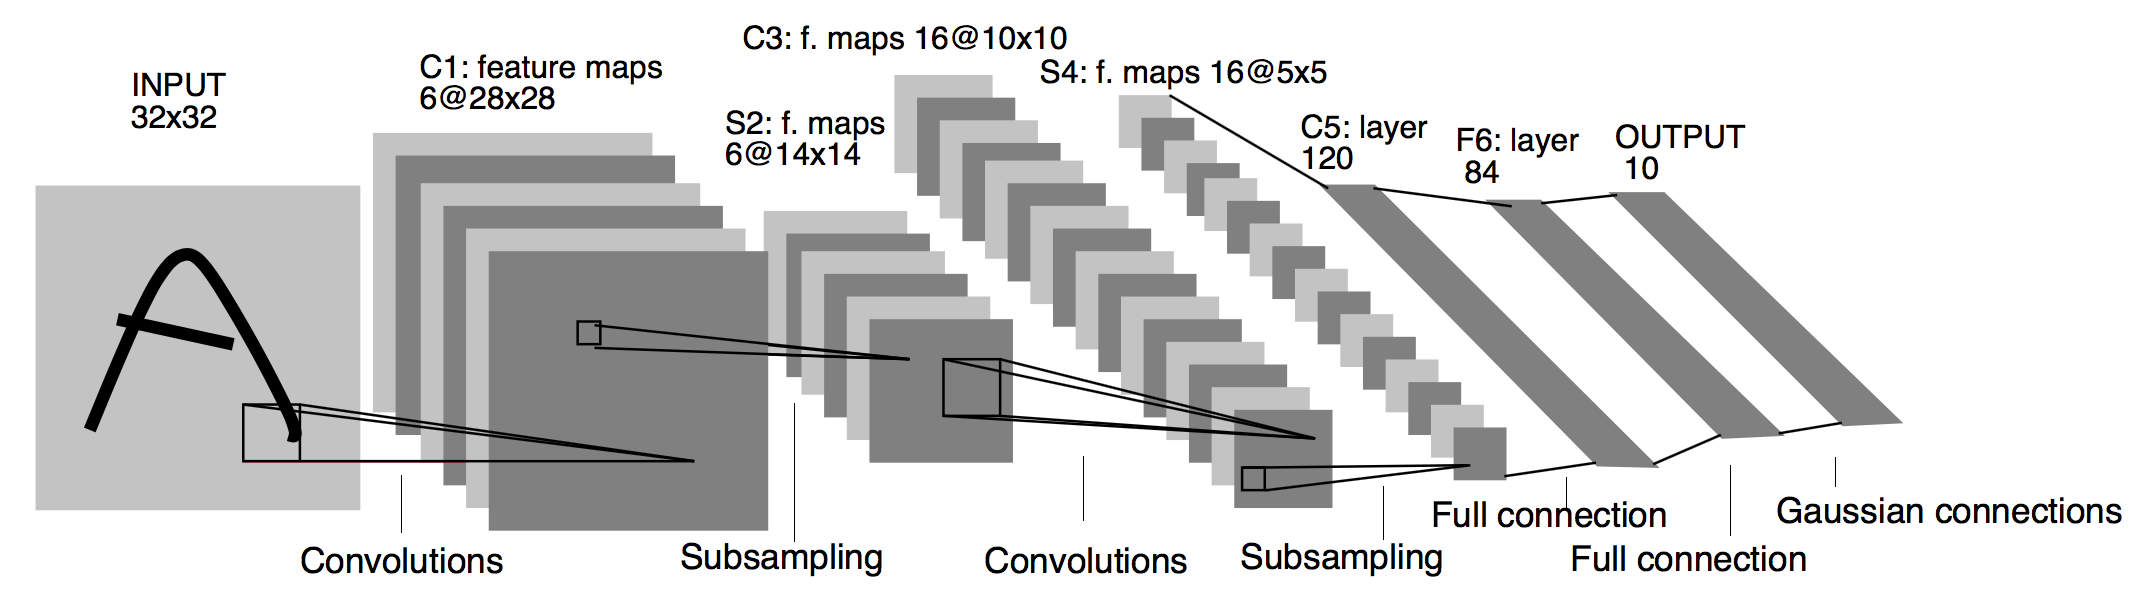
\includegraphics[width=0.5\textwidth]{figs/lenet.png}
    \caption{LeNet}
    \label{fig:lenet}
\end{figure}

AlexNet \cite{alexnet} won the \ac{ILSVRC} \cite{imagenet} in 2012 by a very large margin, introducing a breakthrough in computer vision which further proved that learned features could be better than hand-designed features chosen heuristically. The network, pictured in figure \ref{fig:alexnet}, employed an 8-layer \ac{CNN} that stacked many convolutional layers (immediatelly followed by pooling layers) producing progressively smaller convolutional windows, topped off by two fully-connected layers with 4096 outputs and finally a softmax layer for classification in ImageNet. In its design they also used Dropout regularization and the ReLU activation function, which today are very popular and essential tools in deep learning.

\begin{figure}[ht]
    \centering
    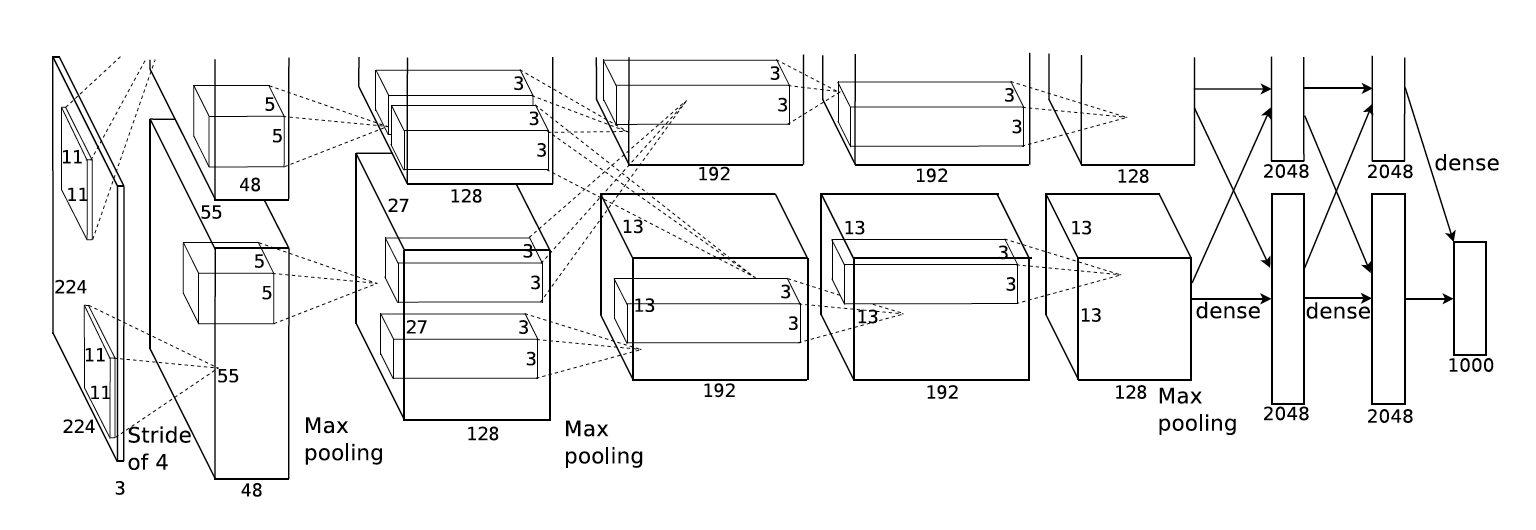
\includegraphics[width=0.6\textwidth]{figs/alexnet.png}
    \caption{AlexNet}
    \label{fig:alexnet}
\end{figure}

Later the \ac{VGG} designed an architecture (illustrated in figure \ref{fig:vgg16}) that used repeated blocks of layers to build progressively more abstract features, shifting thinking in terms of layers to blocks. This basic building block consists of a convolutional layer with padding to maintain resolution, a nonlinearity (i.e. ReLU), pooling for downsampling the features. In the original VGG16 paper \cite{vgg16} the authors employed $3 \times 3$ convolutions and $2 \times 2$ max pooling with stride $S = 2$, essentially halving the resolution after each one of these blocks.

\begin{figure}[ht]
    \centering
    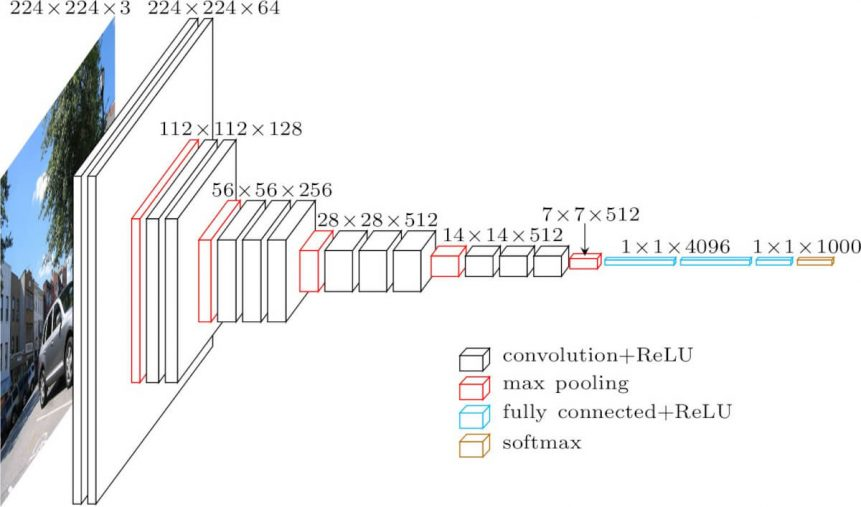
\includegraphics[width=0.6\textwidth]{figs/vgg16.jpg}
    \caption{VGG16}
    \label{fig:vgg16}
\end{figure}

GoogLeNet \cite{inceptionv1} (also known as Inception V1) won the \ac{ILSVRC} \cite{imagenet} in 2014 which introduced the Inception block that establishes four parallel paths that use convolutional layers of different windows and max pooling layers. Furthermore it exhibited lower computational complexity when compared to other models with similar generalization performance. This influenced many later versions of Inception \cite{inceptionv2_3}\cite{inceptionv4}, namely Inception V3 as illustrated in figure \ref{fig:inceptionv3}.

\begin{figure}[ht]
    \centering
    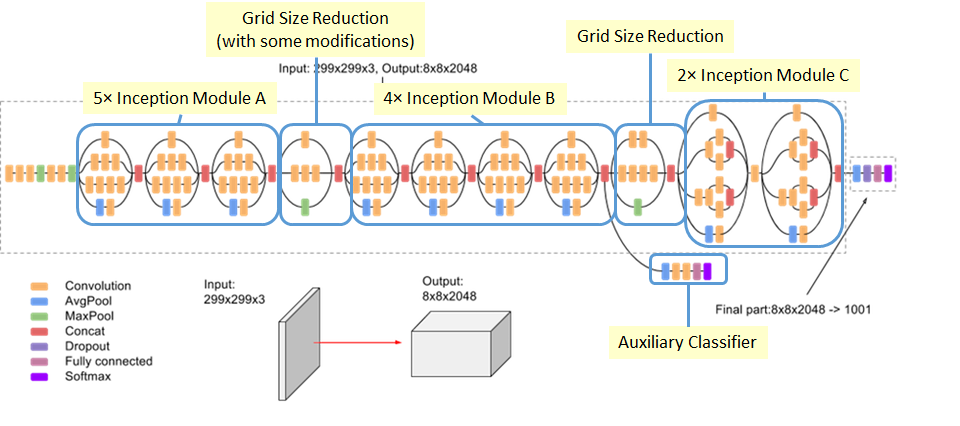
\includegraphics[width=0.6\textwidth]{figs/inceptionv3.png}
    \caption{Inception V3}
    \label{fig:inceptionv3}
\end{figure}

More recently \citeauthor{resnet} have pushed the state-of-the-art by introducing residual neural networks \cite{resnet}. Motivated by avoiding the problem of vanishing gradients, residual networks allow the use of skip connections (or short cuts, as pictured in figure \ref{fig:resnet50}) to arbitrarily jump over layers (effectively reusing activations from previous layers in its forward pass) which significantly speeds up learning by reducing the impact of vanishing gradients since there are less layers to backpropagate through. An ensemble of these networks achieved 3.57\% error on ImageNet, a result which won 1st place on \ac{ILSVRC} 2015.

\begin{figure}[ht]
    \centering
    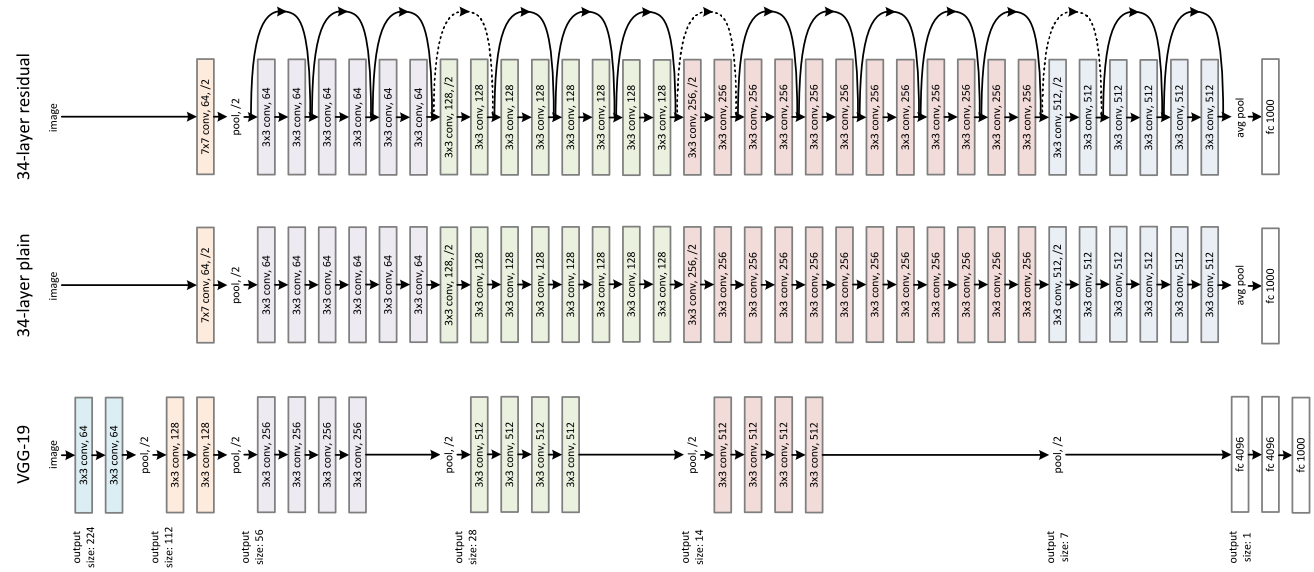
\includegraphics[width=0.7\textwidth]{figs/resnet50.png}
    \caption{Comparison between ResNet-50 and more traditional architectures, illustrating how residual networks avoid the vanishing gradient problem.}
    \label{fig:resnet50}
\end{figure}

\section{Transfer Learning}
\label{section:transferlearning}

Supervised training of deep neural networks requires vast amounts of labeled data, which is very expensive and time consuming in itself, as well as immense computational and time resources which is often equally or more expensive. In practice, transfer learning emerges as a technique that can be used to reduce the costs or time constraints of training these deep neural networks.

Transfer learning is a machine learning technique that seeks to leverage (or transfer) the knowledge gained from solving one problem to another (ideally related) problem \cite{deeptransferlearning}. In the context of deep neural networks it means to transfer the weights of a model trained on a very large dataset (e.g. ImageNet \cite{imagenet}) and re-purpose them for another model.

In image classification problems \ac{CNN} models are used to build progressively more specific feature maps in layers, where lower layers represent abstract, problem independent features (e.g. squares, circles) and higher layers represent specific, problem dependent features (e.g. car, dog). Transfer learning seeks to exploit and take advantage of this construct. In practice, transfer learning for current state-of-the-art image classification techniques boils down to:

\begin{enumerate}
    \item choosing up to which layers should features be extracted
    \item connecting it to a classifier
    \item deciding which layers' weights should be trained (i.e. updated during gradient descent) and which should remain frozen (i.e. not updated during gradient descent)
\end{enumerate}

The classifier is commonly based on:

\begin{itemize}
    \item Fully connected layers;
    \item Global average pooling;
    \item SVM.
\end{itemize}

\subsection{Transfer Learning by Total Feature Extraction}

In the simplest scenario:

\begin{enumerate}
    \item extract all the convolutional layers of the pre-trained model
    \item freeze the weights of all the extracted layers
    \item build a classifier on top of the extracted features and only train the weights of the classifier layers
\end{enumerate}

\subsection{Transfer Learning by Partial Feature Extraction}

When the source and target domains are not very similar, extracting higher layers will yield features that are too specific to the source domain. For example, if the source domain is cars but the target domain is dogs, then the higher layers likely represent features very specific to dogs (e.g. dog eyes, dog tails, dog legs), whereas some arbitrary middle layer might represent more abstract shape-like features that can still be used as a solid starting point for the cars domain.

For this reason it is often counter-productive to extract all the features. Instead features can be extracted up to an arbitrary middle layer which likely represents more useful features that are still relevant for the target domain. The precise point up to which features should be extracted needs to be studied and tested empirically for each problem and chosen based on whichever yields the highest generalization performance.

Like the previous strategy, the classifier is built on top of the extracted features and only the weights of the classifier layers are trained.

\subsection{Transfer Learning by Fine-Tuning}

The weights of the extracted layers (regardless if they were all extracted or only partially) do not all need to remain frozen. Given sufficient computational and time resources, further training the weights of the extracted layers can yield even higher generalization performance because we are, in some sense, fine-tuning the weights of the extracted features to better fit the target dataset.

For this fine-tuning one should be very careful and make sure to use a very slow (i.e. low) learning rate so as to not suddenly disrupt the learned features, because we are actually updating weights transferred from another model.

\section{Ensemble Learning}

Ensemble learning is a machine learning paradigm that designs models by combining other models into a single more complex and presumably more accurate model. In ensemble learning theory we refer to these building block models as weak learners because they usually suffer from high bias or high variance, which are combined in such a way to reduce the bias and variance into a final ensemble model called a strong learner.

There are three major ensemble learning methods: bagging, boosting, and stacking.

\subsection{Bagging}

Bagging, short for bootstrap aggregation, focuses on reducing variance and relies on $L$ approximately i.i.d. subsamples of the data (called bootstrap samples) to fit $L$ weak learners $h_1(x), h_2(x), \ldots, h_L(x)$ and aggregate or average them through some function $H(x)$ which e.g.

\begin{enumerate}
    \item in a regression problem can literally be the average of the predictions of the weak learners, sometimes referred to as soft voting, i.e. $H(x) = \frac{1}{L} \sum_{i=1}^{L} h_i(x)$
    \item in a classification problem can be to just take the mode of the predictions of the weak learners, often called hard voting, i.e. $H(x) = \mode{(h_1(x), h_2(x), \ldots, h_L(x))}$
\end{enumerate}

Perhaps the biggest advantage of bagging is that the the $L$ weak learners can be fit independently and in parallel, considerably speeding up research iterations.

\subsection{Boosting}

Boosting fits multiple models sequentially such that the model being fit at a given iteration gives more importance to samples that were previously predicted with high error, thus resulting in a strong learner with lower bias than its weak learners.

Adaptive boosting (also known as AdaBoost) \cite{adaboost} combines the output of its $T$ weak learners into a weighted sum that represents the final output and is of the form

$$
H_T(x) = \sum_{t=1}^{T} \alpha_t h_t
$$

Rather than optimizing for the optimal set of weights $\alpha_t$ and weak learners $h_t$, AdaBoost takes an iterative approach. Essentially, at each iteration $t$, a weak learner $h_t$ is chosen and weighted $\alpha_t$ to minimize the training error $E_t$ of the $t$-th boosting classifier

$$
E_t = \sum_{t=1}^{T} E[H_{t-1}(x_t) + \alpha_t h_t(x_i)]
$$

\subsection{Stacking}

Rather than combining the weak learners using some arbitrary pre-determined scheme, stacking learns this combination by training a meta-model based on the weak learners' predictions, which can even be done in multiple layers.

Stacking often works well with heterogeneous weak learners, i.e. different algorithms. For example, our weak learners could consist of \ac{KNN}, \ac{SVM}, and decision tree models. Then, the outputs of the weak learners could be taken as inputs for an \ac{ANN} to learn the meta-model based on their predictions.

The data that is used to train the weak learners is not relevant for training the meta-model. Thus we need to split the data in two folds: one for training the weak learners and another for training the meta-model. An obvious immediate drawback is that we only have a fraction of the data available for training the meta-model and vice versa.

\section{Deep Learning Hardware}

Deep learning is very computationally intensive in itself and even more so when we want to run multiple experiments with hyperparameters or even completely different architectures.

\ac{CNN}, the core of most state-of-the-art deep learning applied to computer vision, are computationally complex and embarassingly parallel \cite{chang2017} which the architecture of general purpose \ac{GPU} are appropriate for \cite{gpu} and for which libraries like cuDNN \cite{cudnn} were developed to further leverage the characteristics of \ac{GPU} into even bigger performance improvements.

There is a growing demand for domain-specific hardware designed specifically for the computations necessary in neural network training and inference, like Google's TPU custom ASIC \cite{tpu}, which naturally can achieve major improvements in cost-energy-performance when compared to general purpose hardware like \ac{GPU} that were originally designed for the demands of computer graphics which coincidentally also serve deep learning reasonably well. Nonetheless, \ac{GPU} remain the best cost-effective commodity hardware for this type of computation, especially when not working at the scale of companies like Google and Facebook. In a typical scenario, the CPU does little useful computation in a deep learning application where most of the computation is delegated to the GPU.

% TODO: write more

\section{Deep Learning Software Frameworks}

TensorFlow is an open source software library for numerical computation using data flow graphs. The graph nodes represent mathematical operations, while the graph edges represent the tensors that flow between them. This flexible architecture enables you to deploy computation to one or more CPU or GPU in a desktop, server, or mobile device without rewriting code \cite{tensorflow}.

Keras is a high-level neural networks API, written in Python and capable of running on top of TensorFlow, CNTK or Theano. It was developed with a focus on fast experimentation which enables easy and fast prototyping through user friendliness, modularity, and extensibility. This API was more recently adopted by TensorFlow itself in the tf.keras namespace which is given a lot more attention in TensorFlow 2.0 (following the criticism of TensorFlow's convoluted API).

% TODO: write more
